\subsection*{Algorithmik}

Als Format für die Datenbasis wurde sich für GeoJSON als Standard-/Format \cite{butlerGeoJSONFormat2016} verwendet. Es ist ein weitverbreitetes und offenes Format, das die Beschreibung geografischer Daten ermöglicht. Es wurde für den Zweck der besseren Benutzung in ein eigenes einheitliches Format überführt. Hierbei sind nur leichte Anpassungen entstanden. Die größten Änderungen waren dabei, die Koordinaten nicht als Array, sondern als Objekt zu speichern. Dies erleichtert die Verarbeitung der Daten, wie der Zugriff über den Namen (Value) und nicht über den Index erfolgt.

\begin{lstlisting}[caption={Zugriff über Index oder Value},label={lst:replaceCode}, language=javascript]
// Zugriff über Index
feature.geometry.coordinate[0]

// Zugriff über Value
feature.geometry.coordinate.lat;
\end{lstlisting}


Dies ist besonders entscheidend, da die Reihenfolge von lat und lon nicht einheitlich ist. Mit der Verwendung des Objektes ist der Zugriff immer eindeutig.

Ein wichtiger Faktor ist die Recheneffizienz. Um diese zu erhöhen, werden nur relevante Zonen betrachtet. Hierfür wird eine Bounding-Box um die Route und die Zonen gelegt. Wenn die Bounding-Box der Route eine Bounding-Box der Zonen schneidet, wird die Zone betrachtet, ansonsten nicht. Dies reduziert die Anzahl der zu betrachtenden Zonen erheblich und erhöht somit die Recheneffizienz.

\begin{center}
    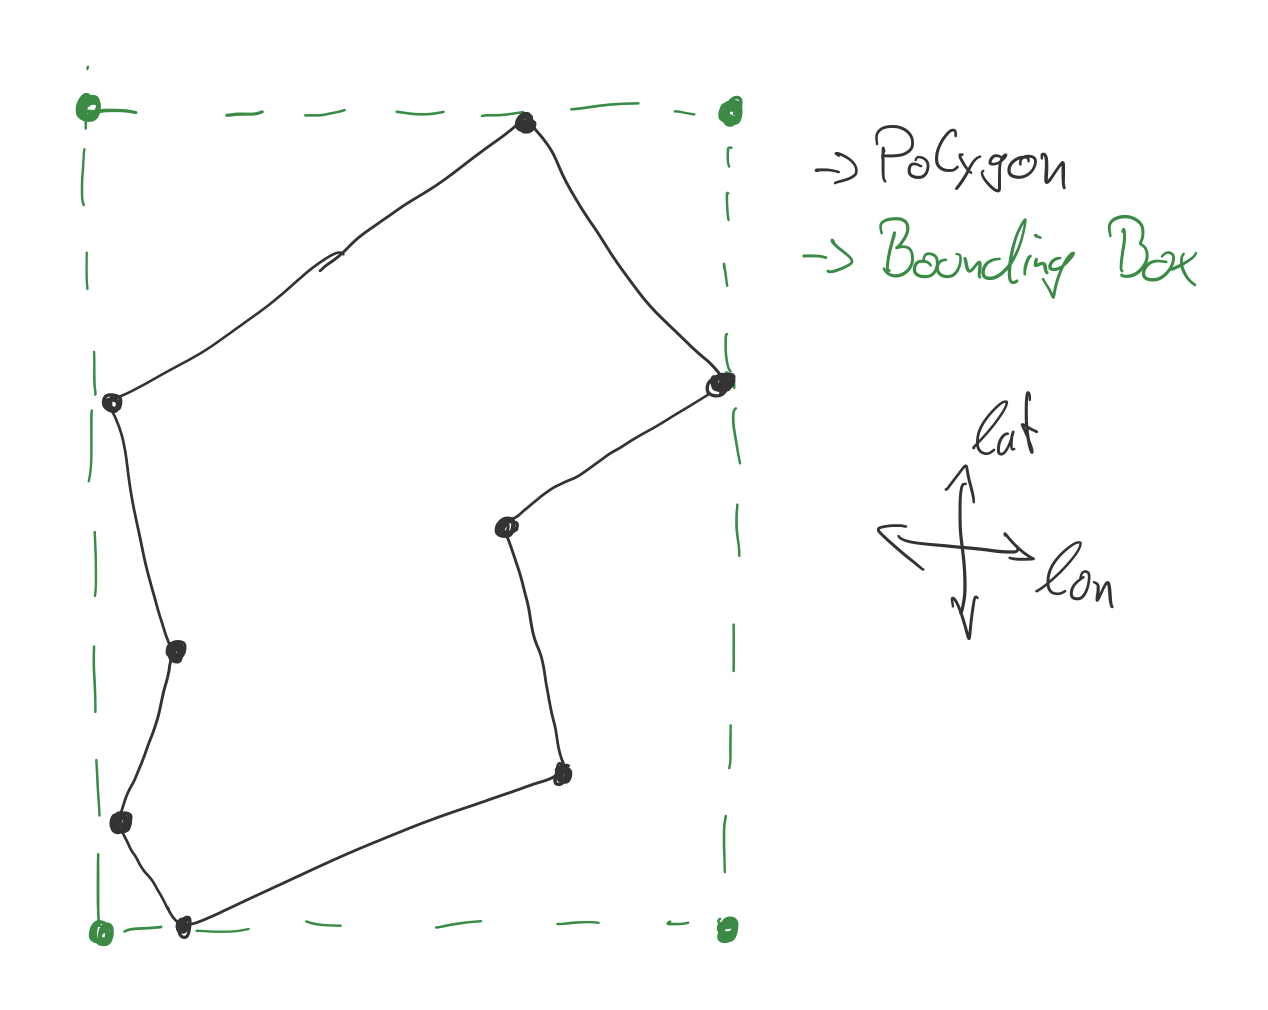
\includegraphics[width=\columnwidth]{images/boundingbox}
    \captionof{figure}{Bounding-Box}
\end{center}

OpenTopoData wird als Datenquelle für die Höhendaten verwendet. Die Route wird in kleinen Abständen abgetastet, dabei wird versucht, innerhalb des Korridors (min - max Flughöhe) möglichst gerade zu fliegen. Dies reduziert die Anzahl der Höhenkorrekturen.

Es gibt jedoch auch offene Probleme, die gelöst werden müssen. Ein Problem ist die Behandlung von konkaven Geometrien von Zonen.

\begin{center}
    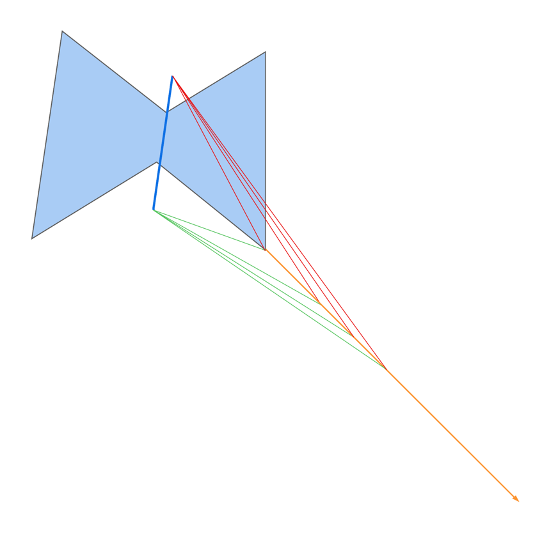
\includegraphics[width=\columnwidth]{images/konkaves-problem}
    \captionof{figure}{Konkaves Problem}
\end{center}

Hier landet ein Routenpunkt in einer konkaven Geometrie einer Zone und der Algorithmus läuft ins Unendliche. Es gibt bereits verschiedene Lösungsansätze wie den A*-Algorithmus \cite{Algorithmus2022}, IDA* \cite{IDA2021} oder indem Eckpunkte der Zone als Zwischenpunkte eingebaut werden, um dem Konkaven zu entkommen.

Ein weiteres Problem ist die Optimierung der Route. Derzeit wird der erstbeste Weg genommen, dieser ist jedoch nicht zwingend der effizienteste. Hier können verschiedene Optimierungsverfahren angewendet werden, um die Routeneffizienz zu verbessern.

\begin{center}
    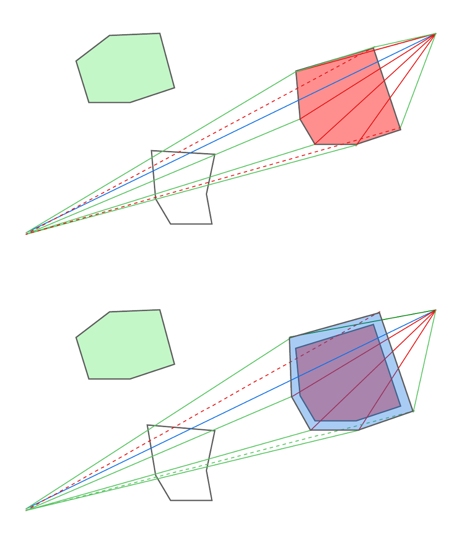
\includegraphics[width=\columnwidth]{images/routing-algo}
    \captionof{figure}{Routing Algorithmus}
\end{center}